\chapter{Benchmark und Bewertung}
\label{chapter:Dokumentation-BenchmarkBewertung}

\section{Berechnung}
\label{section:Dokumentation-BenchmarkBewertung-Berechnung}

Für die Berechnung der Laufzeit, der Länge und für die Bewertung des Algorithmus gelten folgende Vorschriften:

\subsection{Variablen}
\label{subsection:Dokumentation-BenchmarkBewertung-Berechnung-Variablen}

\begin{description}
    \item[reg] Anzahl der ergänzten Minimaxregister
    \item[se] Anzahl der ergänzten Sign"=Extension"=Units (0 oder 1)
    \item[const] Anzahl der ergänzten Konstanten (eine "`0"' und eine "`1"' frei)
    \item[alu\_add] Penaltysumme für alle ergänzten ALU"=Befehle
    \item[alu\_use] Penaltysumme der \emph{verwendeten} ALU"=Befehle im Programm
\end{description}

\begin{center}
    \begin{tabular}{|@{\hspace{2pt}}c@{\hspace{2pt}}||@{\hspace{2pt}}c@{\hspace{2pt}}|@{\hspace{2pt}}c@{\hspace{2pt}}|@{\hspace{2pt}}c@{\hspace{2pt}}|@{\hspace{2pt}}c@{\hspace{2pt}}|@{\hspace{2pt}}c@{\hspace{2pt}}|@{\hspace{2pt}}c@{\hspace{2pt}}|@{\hspace{2pt}}c@{\hspace{2pt}}|@{\hspace{2pt}}c@{\hspace{2pt}}|}
        \hline
        extra ALU"=Op. & SUB1 & INC/DEC & S.L, S.R & AND, OR, NOT & XOR & DIV & MUL & Custom \\ 
        \hline
        Penalty (1..20) & 1 & 4 & 5 & 6 & 8 & 10 & 16 & bis zu 20 \\
        \hline
    \end{tabular}
\end{center}

\subsubsection{Variablenwerte}
\label{subsubsection:Dokumentation-BenchmarkBewertung-Berechnung-Variablen-Variablenwerte}

Im Folgenden sind die Werte für den verwendeten Algoritmus angegeben:

\begin{align*}
    reg      &= 6 \\
    se       &= 0 \\
    const    &= 7 \\ \\
    alu\_add &= MUL + AND + SR.B \\
             &= 16 + 6 + 5 = 27 \\ \\
    alu\_use &= 4 \cdot MUL + 6 \cdot AND + 14 \cdot SR.B \\
             &= 4 \cdot 16 + 6 \cdot 6 + 14 \cdot 5 = 170
\end{align*}

\subsection{Laufzeit}
\label{subsection:Dokumentation-BenchmarkBewertung-Berechnung-Laufzeit}

Die Laufzeit des Algorithmus wird in Minimaxtakten gezählt und berechnet sich nach folgender Formel:

\begin{align*}
    t_{bewertet} &= t_{bench} \cdot (1 + 0.1 \cdot reg + 0.15 \cdot se + 0.015 \cdot alu\_add + 0.05 \cdot const) \\
                 &= t_{bench} \cdot (1 + 0.1 \cdot 6 + 0.15 \cdot 0 + 0.015 \cdot 27 + 0.05 \cdot 7) \\
                 &= t_{bench} \cdot 2.355
\end{align*}

Zur Bestimmung von $t_{bench}$ wurden 3 Speicherabbilder mit jeweils 1120 Bytes zur Verfügung gestellt:

\begin{enumerate}
    \item Alle Pakete haben eine Länge von 80 Bits (Pakete ohne Daten)
    \item Durchschnittliche Datenteillänge von 80 Bits
    \item Durchschnittliche Datenteillänge von 144 Bits
\end{enumerate}

Nach Simulation des Algorithmus mit allen drei Beispielen wurden folgende Ergebnisse festgestellt:

\begin{center}
    \begin{tabular}{|l|l|r|}
        \hline
        Speicherabbild & Minimaxtakte & \multicolumn{1}{l|}{$t_{bewertet}$} \\
        \hline
        \hline
        1 & 24\,935 & 58\,721.925 \\
        \hline
        2 & 58\,423 & 137\,586.165 \\
        \hline
        3 & 67\,975 & 160\,081.125 \\
        \hline
    \end{tabular}
\end{center}

\begin{multicols}{3}
    Benchmark 1:
    
    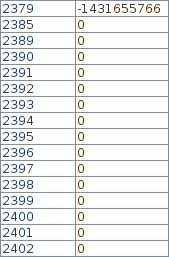
\includegraphics[width=0.25\textwidth]{dokumentation/res/bench1_result.png}
    \vfill
    \columnbreak
    
    Benchmark 2:
    
    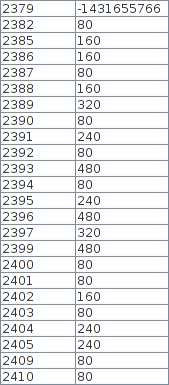
\includegraphics[width=0.25\textwidth]{dokumentation/res/bench2_result.png}
    \vfill
    \columnbreak
    
    Benchmark 3:
    
    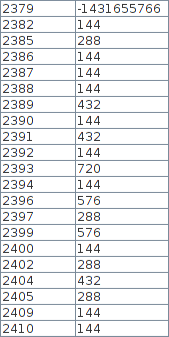
\includegraphics[width=0.25\textwidth]{dokumentation/res/bench3_result.png}
\end{multicols}

\subsection{Länge}
\label{subsection:Dokumentation-BenchmarkBewertung-Berechnung-Laenge}

Die Länge des Algorithmus berechnet sich nach folgender Formel:

\begin{align*}
    n_{bewertet} &= n_{Algorithmus} + 5 \cdot reg + 10 \cdot se + 3 \cdot alu\_use + 5 \cdot const \\
                 &= 118 + 5 \cdot 6 + 10 \cdot 0 + 3 \cdot 170 + 5 \cdot 7 \\
                 &= 118 + 575 \\
                 &= 693
\end{align*}

\section{Abschließende Bewertung}
\label{section:Dokumentation-BenchmarkBewertung-Bewertung}

Dieser Algorithmus überzeugt hauptsächlich durch den einfachen Zugriff auf das Ergebnis. Da der Hauptspeicher unbegrenzt ist, stellt der große Bruttospeicherbedarf keinen allzu großen Nachteil dar. Die Laufzeit des Algorithmus ist der Aufgabe angemessen, wäre aber mit einem mächtigeren Simulator deutlich niedriger. Viele Implentierungen stellen Workarounds für Probleme dar, die erst durch den Simulator entstanden sind (wie z.B. unbedingte Sprünge). Die umfangreichen Hardwareerweiterungen erfordern eine ausreichend hohe Auflagengröße, da nicht vollständig auf Standardkomponenten zurückgegriffen werden kann. Für kleinere Stückzahlen findet sich eventuell eine umfangreichere Basismaschine, wodurch die Kosten eventuell reduziert werden können.

\section{Probleme bei der Durchführung}
\label{section:Dokumentation-BenchmarkBewertung-Probleme}

Während der Entwicklung nahm die Implementierung für den Simulator die meiste Zeit in Anspruch. Das Verhalten war mehrfach unerwartet und undokumentiert. Fehlermeldungen bestanden i.d.R. lediglich aus Stacktraces, welche ohne den Quelltext jedoch weitgehend nutzlos waren. Hier sind Fehler aufgelistet, auf die wir gestoßen sind.

\begin{itemize}
    \item Multiplikation produziert Overflows und schneidet nicht einfach ab
    \item Strings in der GUI sind nicht ausgeschrieben
    \item Multiplexer A hat maximal 12 Eingänge (trotz theoretischer 4 Bit)
    \item Multiplexer B hat maximal 9 Eingänge (trotz theoretischer 4 Bit)
    \item if geht nur mit else
    \item Leitungen lassen sich nicht teilen
    \item Fehlermeldungen (Stacktrace) unbrauchbar, da kein Quelltext vorhanden ist
    \item kann nicht vorzeichenlos durch 2 teilen (Shiftersatz)\footnote{Beispiel:\\
\texttt{
999a6666 / 2\\
10011001100110100110011001100110\\
cccd3333 Simulator\\
11001100110011010011001100110011\\
4ccd3333 Wolfram Alpha\\
01001100110011010011001100110011}}
    \item unbedingte Sprünge nicht möglich
    \item Simulator ignoriert Leerzeichen nicht
    \item keine Kommentare am Zeilenende
\end{itemize}
